\newpage
\chapter {Specifica di Dettaglio}

Di seguito verrà fornita una descrizione dell'architettura del progetto realizzato, e in particolare verrà descritto come le soluzioni progettate sono state realizzate nella pratica.

\section{Simulazione}

	\begin{figure}[htbp]
		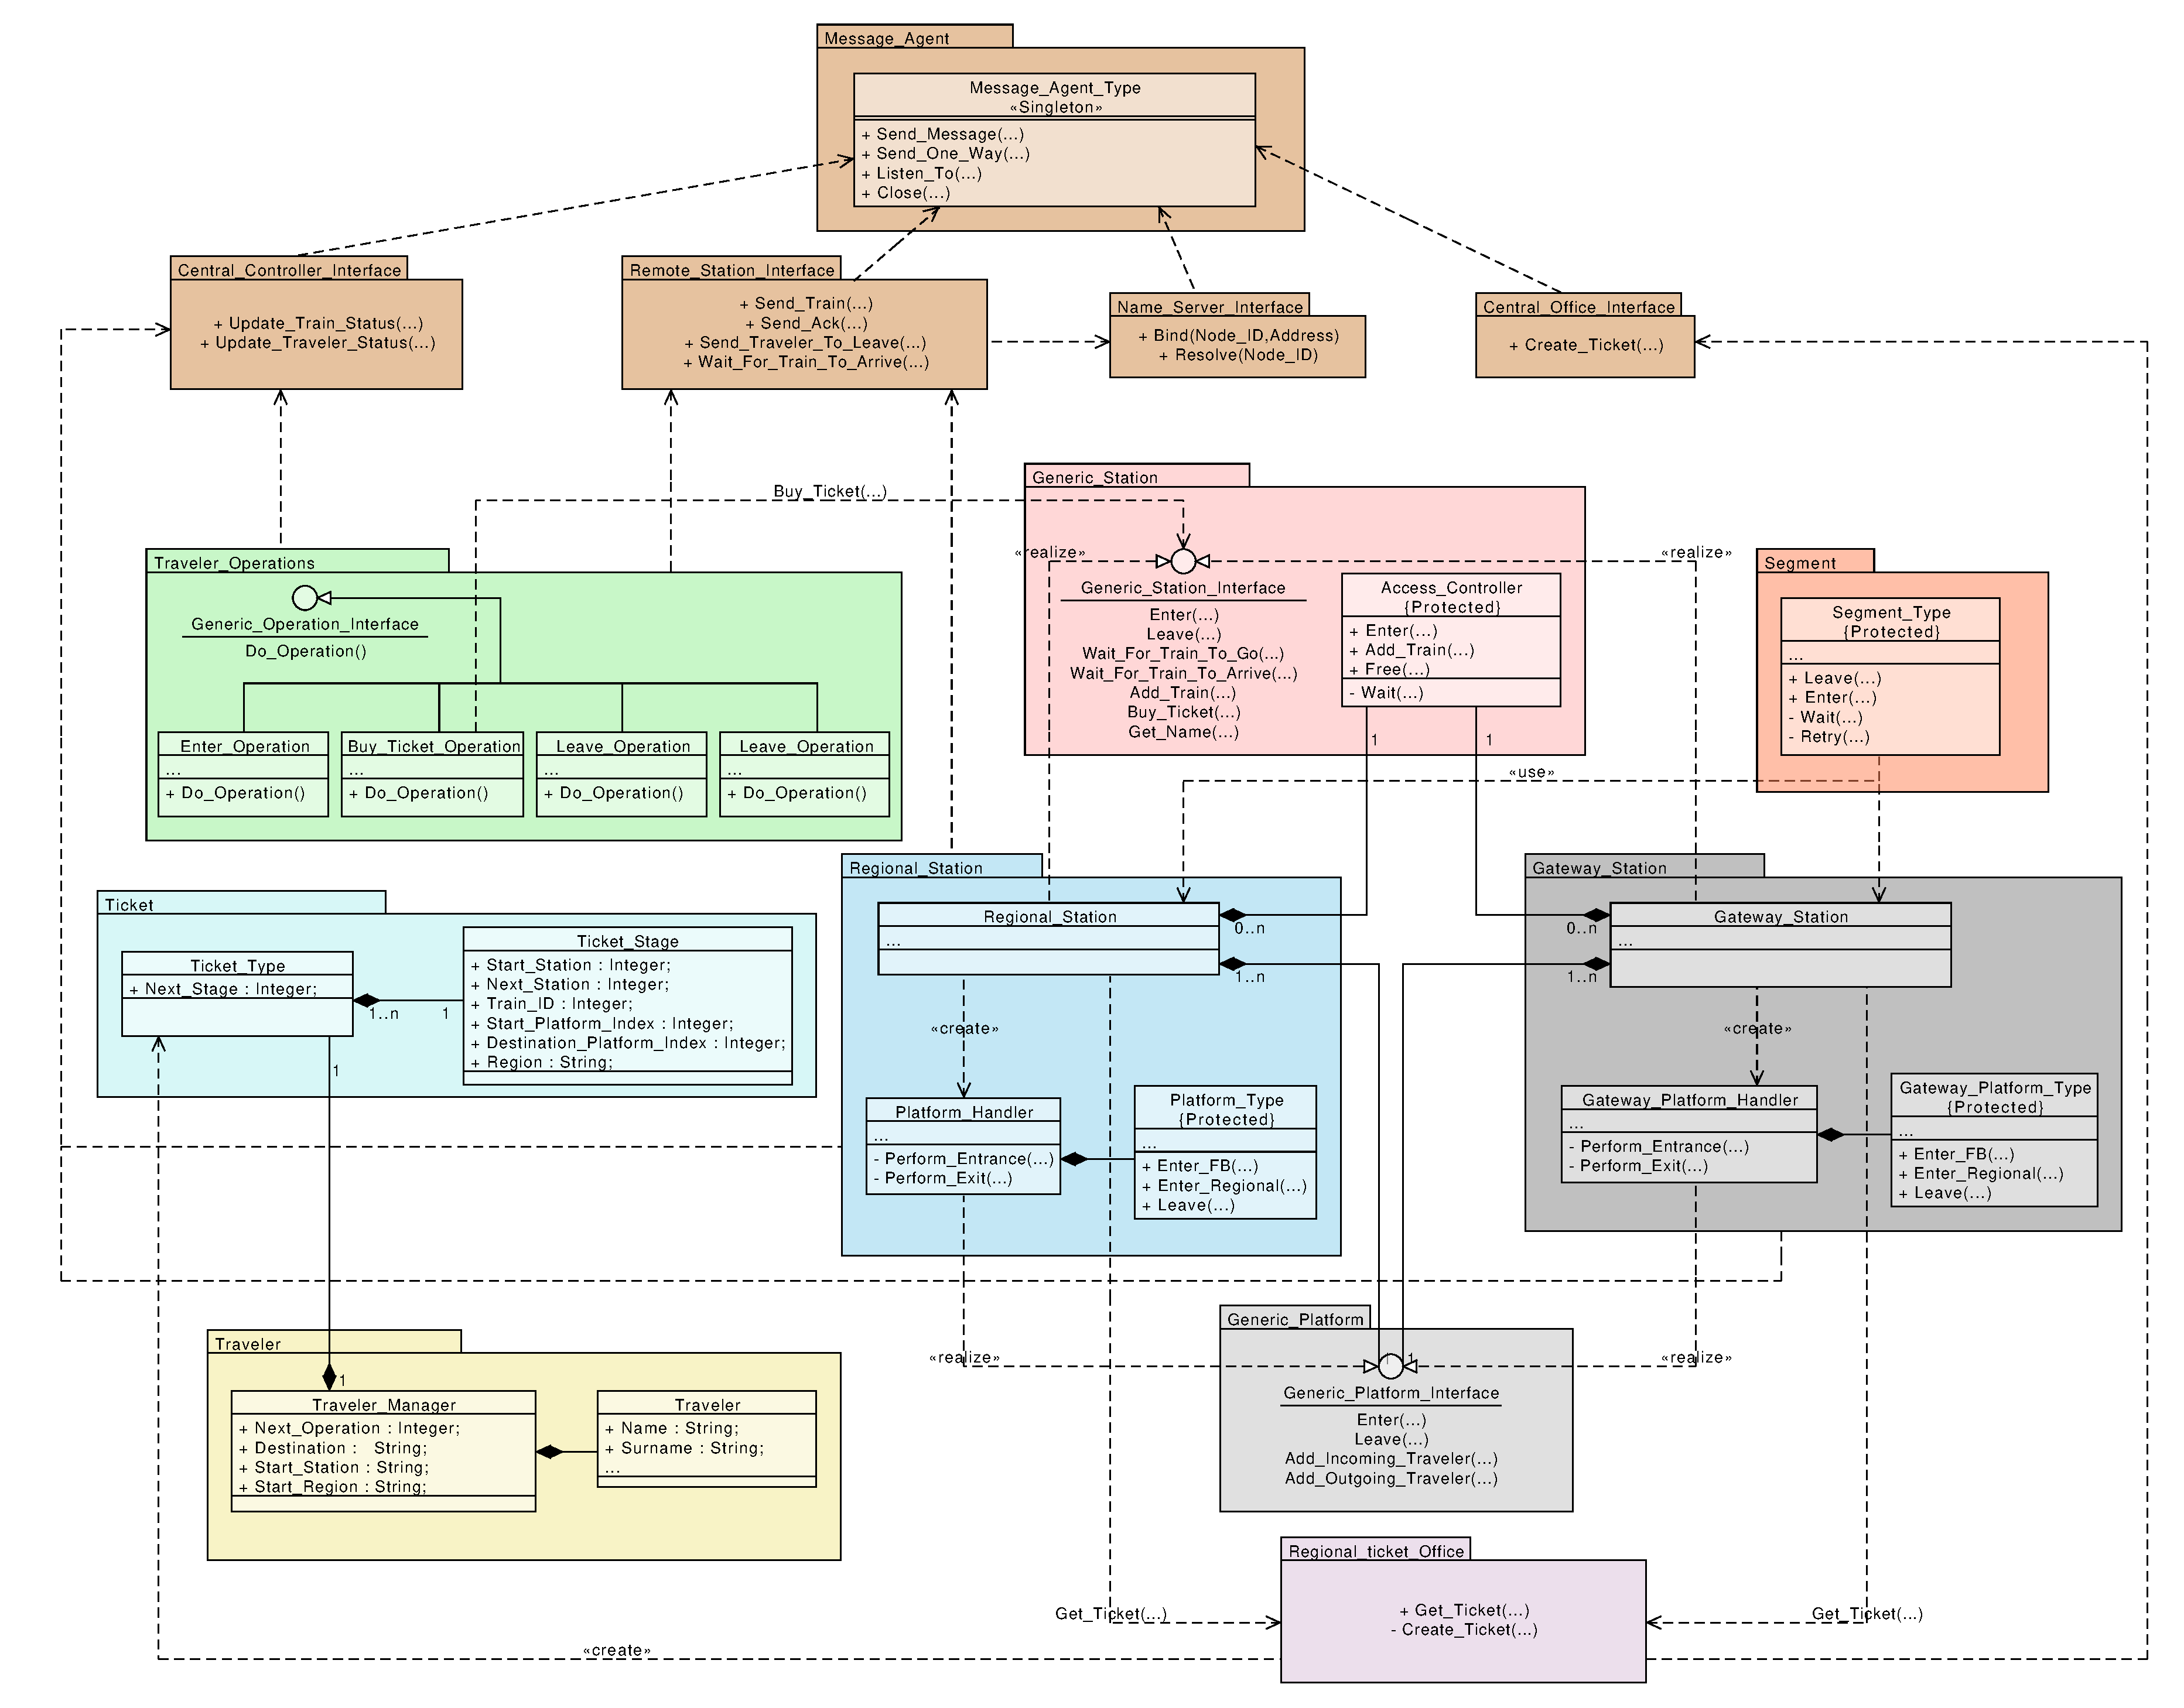
\includegraphics[scale=0.32,trim= 100mm 0mm 0mm 0mm]{imgs/Class_Diagram_2.pdf}
		\caption{\footnotesize{Diagramma delle classi che illustra le componenti e le relazioni più significative che coinvolgono la simulazione.}}
		\label{img:class_diagram}
	\end{figure}

L'architettura di massima adottata per la realizzazione del core di simulazione, è visibile nel diagramma delle classi in figura \ref{img:class_diagram} nel quale, per brevità, sono stati riportati solo le informazioni più significative.
	Viene ora fornita una descrizione delle varie componenti Package. Nelle sezioni seguenti si utilizzeranno le nozioni di \ii{Task} e \ii{Tipo protetto} definite dal linguaggio \ii{Ada} utilizzato per la realizzazione delle componenti di simulazione del sistema. 

	\subsection{Message\_Agent}
	
	Il package \ttt{Message\_Agent} fornisce un'interfaccia per l'invio di messaggi remoti. Esso contiene una classe singleton \ttt{Message\_Agent\_Type}, la quale possiede i seguenti campi dato:
	\begin{description}
		\item \ttt{- Client\_Agent : YAMI.Agents.Agent\_Access} \\
		Campo dati privato di tipo \ttt{YAMI.Agents.Agent\_Access} che contiene una istanza di Agente fornito dalla libreria \ii{Yami4}, e che viene utilizzato per l'invio e la ricezione di messaggi remoti.
		\item \ttt{- Handlers\_Map : Map} \\
		Hash-map privata, la quale associa a chiavi di tipo \ttt{String}, valori di tipo \ii{riferimento a procedura}; essa viene utilizzata per associare a ciascun servizio offerto dall'oggetto \ttt{Client\_Agent} un handler per la sua gestione.
	\end{description}
	
	Essa offre inoltre i seguenti metodi:
	
	\begin{description}
		\item \ttt{+ Listen\_To(Server\_Address)} \\
		Indica all'oggetto \ttt{Client\_Agent} di rimanere in ascolto presso l'indirizzo \ttt{Server\_Address}, attraverso il quale riceverà tutti i messaggi destinati al nodo. Nella fase di registrazione dell'oggetto remoto, viene definito un handler per la ricezione dei messaggi, il quale effettua il dispatching del messaggio invocando la procedura corrispondente al servizio richiesto, definita nella mappa \ttt{Handlers\_Map}.
		
		\item \ttt{+ Close()} \\
		Chiude la connessione dell'oggetto \ttt{Client\_Agent}.
		
		\item \ttt{+ Send\_Message(\\
			Destination\_Address:String,\\
			Object:String,\\
			Service:String,\\
			Params:YAMI.Parameters.Parameters\_Collection,\\
			Callback)}\\
		Invia un messaggio all'oggetto remoto indicato da \ttt{Object} all'indirizzo \ttt{Destination\_Address}, richiedendo il servizio \ttt{Service}, e con i parametri indicati da \ttt{Params}. Se non nulla, la funzione di callback \ttt{Callback} viene invocata alla ricezione del messaggio di risposta, altrimenti quest'ultimo viene ignorato.
		
		\item \ttt{+ Send\_One\_Way(\\
			Destination\_Address : String,\\
			Object 				: String,\\
			Service 			: String,\\
			Params 				: YAMI.Parameters.Parameters\_Collection)}\\
		Metodo simile a \ttt{Send\_Message}, solo che non rimane in attesa della risposta al messaggio inviato.
	\end{description}
	
	Nessun meccanismo di serializzazione delle richieste è stato adottato, in quanto esso è già operato dagli oggetti della libreria \ii{Yami4}.
	
	\subsection{Central\_Controller\_Interface}
	
	Il package \ttt{Central\_Controller\_Interface} fornisce un'interfaccia per permettere alle entità della simulazione di inviare un evento di notifica alla componente remota di Controllo Centrale. A tal proposito sono messi a disposizione le procedure \ttt{Set\_Train\_Status} e \ttt{Set\_Traveler\_Status}, le quali effettuano il marshalling dei dati in ingresso (in formato \ttt{JSON}) e inviano un messaggio remoto mediante il metodo \ttt{Send\_One\_Way} offerto dall'unica istanza di \ttt{Message\_Agent\_Type}.
	
	\subsection{Central\_Office\_Interface}
	
	Il package \ttt{Central\_Office\_Interface} fornisce un'interfaccia per permettere la comunicazione con la Biglietteria Centrale. Per questo è messa a disposizione una procedure \ttt{Create\_Ticket} la quale richiede la creazione di un Biglietto inviando un messaggio remoto mediante il metodo \ttt{Send\_Message} offerto dall'unica istanza di \ttt{Message\_Agent\_Type}. Non viene specificata una procedura di callback, in quanto il risultato verrà inviato dalla Biglietteria Centrale una volta calcolato il Biglietto.
	
	\subsection{Name\_Server\_Interface}
	
	Package che fornisce un'interfaccia remota per la comunicazione con il Server dei Nomi che mantiene la lista delle Regioni di simulazione. Esso fornisce le seguenti procedure:
	\begin{description}
		\item \ttt{+  Bind(\\
		Name\_Server : String,\\
		Node\_Name 	: String,\\
		Address	: String)} \\
	Permette di registrare presso il Server dei Nomi che l'entità remota \ttt{Node\_Name} è disponibile alla locazione indicata da \ttt{Address}. 
	
	\item \ttt{+  Resolve(\\
		Name\_Server : String,\\
		Node\_Name 	: String),\\
		Callback : access procedure(Result:String)} \\
		Permette di richiedere al Server dei Nomi la risoluzione della locazione alla quale si trova l'entità \ttt{Node\_Name}. Una volta che la risposta è disponibile, viene invocata la procedura di callback \ttt{Callback}. 
				
	\end{description}
	
	Per entrambe le procedure, viene inviato un messaggio remoto tramite il metodo \ttt{Send\_Message} di \ttt{Message\_Agent\_Type}, al quale viene passato una procedura di callback che estrae il campo \ttt{address} dal messaggio di ritorno e lo passa all'invocazione di \ttt{Callback}. Presso il package viene mantenuta una hash-map, la quale permette di memorizzare le destinazioni risolte, in modo da limitare l'invio di messaggi remoti.
	
	\subsection{Queue}
	
	Il package \ttt{Queue} contiene la definizione di alcuni tipi di code utilizzati nell'intera simulazione:
		\begin{description}
			\item {\ttt{Terminable\_Queue}} \\
			Tipo \ii{protetto} costruito come \ii{wrapper} della coda standard offerta dal package \ttt{Ada.Containers.Unbounded\_Synchronized\_Queues}, e che permette di interrompere l'attesa sulla guardia Booleana definita per l'entry \ttt{Dequeue}, la quale rimane chiusa nel caso in cui non vi siano più elementi al suo interno.
			Esso e definisce l'entry
			\begin{center}
				\ttt{Dequeue(Element:out  Element\_Type,Terminated:out  Boolean)}
			\end{center}
		
		con guardia Booleana: \ttt{Termination or Q.Current\_Use > 0}, dove \ttt{Q} è una coda fornita dalle librerie standard di linguaggio, \ttt{Current\_Use} è una funzione che restituisce il numero di elementi all'interno della coda, e \ttt{Termination} è un campo dati Booleano della risorsa protetta. In questo modo nel caso in cui il valore di \ttt{Termination} sia \ttt{True} l'attesa su coda viene interrotta, e viene restituito al chiamante il valore \ttt{True} attraverso il parametro passato per riferimento \ttt{Terminated}, altrimenti la coda restituisce anche il valore del primo elemento rimosso dalla coda.
		
		Per poter attribuire al campo dati \ttt{Termination} il valore \ttt{True}, viene fornita la procedura protetta \ttt{Stop}.
			
			\item {\ttt{Limited\_Simple\_Queue}} \\
			Tipo di coda non thread-safe, di dimensione limitata, realizzato mediante un array di elementi, e che fornisce un'interfaccia composta dai metodi:
			\begin{itemize}
				\item \ttt{Enqueue(Element:Element\_Type)} per accodare un nuovo elemento;
				\item \ttt{Dequeue(Element:out Element\_Type)} per rimuovere l'elemento dalla testa della coda;
				\item \ttt{Get(Index:Integer)} per ottenere il valore dell'elemento nella posizione \ttt{Index};
			\end{itemize}
			
			\item {\ttt{Unlimited\_Simple\_Queue}} \\
			Tipo di coda non thread-safe di dimensione illimitata, realizzato mediante un oggetto di tipo \ttt{Vector} definito dalle librerie standard \ttt{Ada.Containers.Vectors}. Esso presenta un'interfaccia del tutto simile a quella offerta dal tipo \ttt{Limited\_Simple\_Queue}, alla quale aggiunge il metodo \ttt{Is\_Empty : Boolean} che indica se la coda è vuota. 
			
		\end{description}
	
	\subsection{Generic\_Operation\_Interface}
	
	Package che contiene la definizione di una interfaccia \ttt{Operation\_Interface}, la quale espone un unico metodo \ttt{Do\_Operation()}. Essa rappresenta una generica operazione. Viene definito inoltre un tipo puntatore ad operazione generica \ttt{Any\_Operation}.
	
	\subsection{Traveler\_Pool}
	
	Il package {Traveler\_Pool} realizza il meccanismo per l'esecuzione delle entità Viaggiatore descritto in sezione \ref{subsec:traveler_def}. Esso mantiene 
	\begin{itemize}
		\item una coda \ttt{Operations\_Queue} di puntatori di tipo \ttt{Any\_Operation} a operazioni. Tale coda è di tipo \ttt{Terminable\_Queue}, definito nel package \ttt{Queue}.
		\item la definizione di un tipo record \ttt{Traveler\_Pool\_Type} contenente un array di oggetti task \ttt{Executor}, di dimensione fissata in fase di creazione.
		Ciascun task di tipo \ttt{Executor} eseguirà semplici operazioni ciclicamente:
		\begin{itemize}
			\item Estrae il primo elemento dalla coda \ttt{Operations\_Queue} mediante il metodo \ttt{Dequeue} da essa offerto. 
			\item Nel caso in cui il valore del parametro \ttt{Terminated} passato per riferimento abbia il valore \ttt{True}, allora viene interrotto il ciclo di operazioni.
			\item Altrimenti, viene invocato il metodo \ttt{Do\_Operation} sul puntatore ad operazione estratto.
		\end{itemize}
	\end{itemize}
	
	\subsection{Ticket}
	
	Package che contiene la definzione di un Biglietto. Esso definisce infatti il tipo record \ttt{Ticket\_Type}, il quale è composto da un campo intero \ttt{Next\_Stage} che indica la tappa corrente del percorso descritto dal Biglietto, e un puntatore ad un array di Tappe, ovvero di oggetti di tipo \ttt{Ticket\_Stage}. Quest'ultimi mantengono le seguenti infomazioni:
		\begin{itemize}
			\item \ttt{Start\_Station} : Indice della Stazione di partenza;
			\item \ttt{Next\_Station} : Indice della prossima Stazione;
			\item \ttt{Train\_ID} : Identificativo del Treno da utilizzare per raggiungere la stazione \ttt{Next\_Station};
			\item \ttt{Start\_Platform\_Index} : Indice della Piattaforma di partenza;
			\item \ttt{Destination\_Platform\_Index} : Indice della Piattaforma di destinazione;
			\item \ttt{Region} : Nome della regione nella quale si colloca la stazione \ttt{Next\_Station};
		\end{itemize}
	Il package fornisce inoltre le funzioni necessarie per effettuare marshalling e unmarshalling degli oggetti di tipo \ttt{Ticket\_Type} in/dal formato \ttt{JSON}.
	
	\subsection{Traveler}
	
	Package che contiene la definizione del tipo rappresentante un Viaggiatore. In esso infatti viene definito il tipo record \ttt{Traveler\_Manager}, formato dai campi:
		\begin{itemize}
			\item \ttt{Next\_Operation} : Indice della prossima operazione da eseguire;
			\item \ttt{Destination} : Nome della stazione di destinazione;
			\item \ttt{Start\_Station} : Nome della stazione di partenza;
			\item \ttt{Start\_Region} : Regione di patenza;
			\item \ttt{Traveler} : Campo di tipo record che contiene alcuni dati relativi al Viaggiatore, come nome e cognome.
			\item \ttt{Ticket} : Riferimento ad un oggetto di tipo \ttt{Ticket\_Type}.
		\end{itemize}
	Il package \ttt{Traveler} contiene inoltre le funzioni necessarie per effettuare marshalling e unmarshalling secondo il formato \ii{JSON}.
	
	\subsection{Regional\_Ticket\_Office}
	
	Il package \ttt{Regional\_Ticket\_Office} mantiene una tabella \ttt{Paths}, la quale per ciascuna Stazione della Regione corrente, definisce i percorsi più brevi per raggiungere ciascuna altra destinazione nella Regione. Esso inoltre espone un'interfaccia con un unica procedura:
	\begin{center}
	\ttt{Get\_Ticket (Traveler\_Index:Integer,From:String,To:String)} \\
	\end {center}
	la quale si occupa dell'effettiva creazione del Biglietto (oggetto di tipo \\ \ttt{Ticket\_Type}). Tale procedura effettua un controllo: se le Stazioni \ttt{From} e \ttt{To} sono contenute all'interno della Regione corrente, allora procede alla creazione del Biglietto vero e proprio attraverso la funzione privata 
	\begin{center}
		\ttt{Create\_Ticket(From:String,To:String):Ticket\_Type} \\
	\end{center}
che viene quindi assegnato al Viaggiatore di indice \ttt{Traveler\_Index}, e successivamente viene inserita l'operazione \ttt{TICKET\_READY} nella coda di operazioni di \ttt{Traveler\_Pool}. Se invece la Stazione di destinazione \ttt{To} non è contenuta nella Regione corrente, allora viene richiesta la creazione del Biglietto alla Biglietteria Centrale attraverso l'interfaccia \ttt{Central\_Office\_Interface}.
	La funzione \ttt{Create\_Ticket} implementa l'algoritmo di creazione di un oggetto \ttt{Ticket\_Type} descritto in sezione \ref{subsubsec:ticket_creation}.
	
	Il package \ttt{Regional\_Ticket\_Office} contiene inoltre una procedura \\ \ttt{Init\_Path\_Map} per caricare la mappa contenente i percorsi più brevi, utilizzata per l'algoritmo di creazione del Biglietto.
